\begin{recipe}
    [% 
        preparationtime = {\unit[15]{h}},
        portion = {\portion{4}},
        bakingtime = {\unit[25]{min}},
        source = {Jacek}
    ]
    {Chicken in curry coconut milk}

    \ingredients[8]{%
        2 & Chicken breast \\
        2 can & Coconut milk \\
        & Tumeric \\
        & Curry powder \\
        & Paprica \\
        & Coriander  \\
        & Cumin \\
        & Garam masala
    }

    \preparation{%
        \step Cut each breast into 4 elongated pieces.

        \step Toss meat in spices (+salt), line in the oven dish and cover with coconut milk.

        \step Bake for 20-25 min at \unit[180]{\textcelcius}).
        \vspace{1cm}
        \begin{figure}[h]
            \centering
            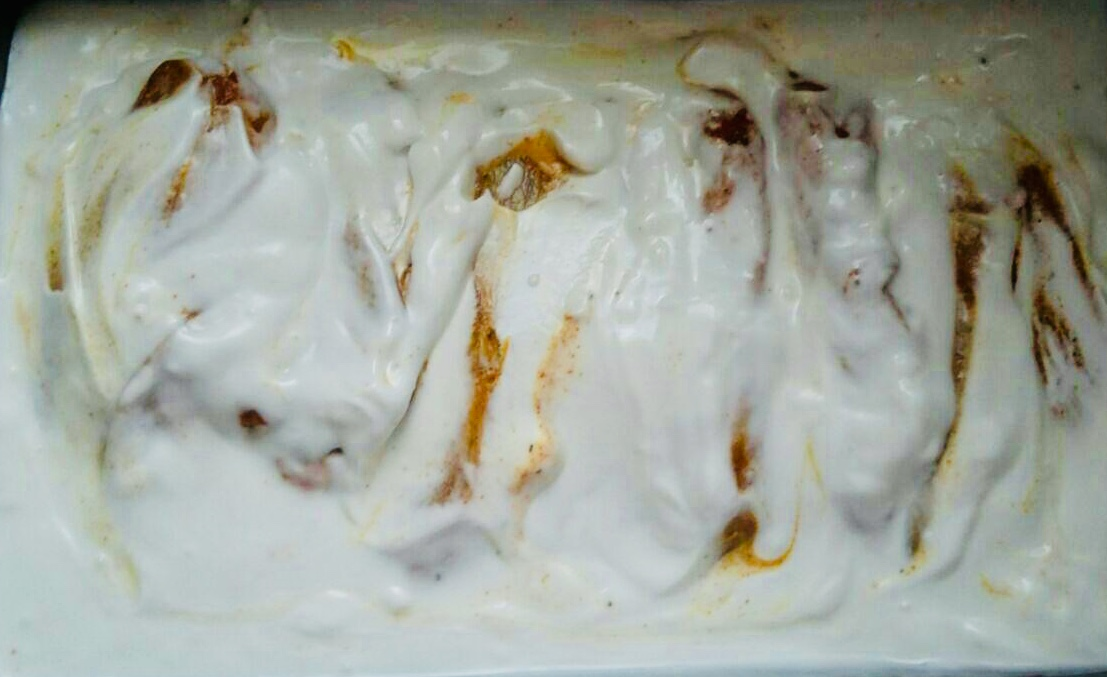
\includegraphics[height=7cm]{pic/coconut_chicken}
        \end{figure}
        % TODO: download extra pic
    }

    \hint{%
        Serve with rice (add lemon juice and coriander leaves) and green beans and peppers fried with garlic and a hint of soy sauce.
    }

\end{recipe}